% !TEX root = ../main.tex
\section{Akhosh} \label{sec::akhosh}
\DndDropCapLine{}{Only victory endures.}

\hspace*{\fill} --- Akhoash motto.

The walled polis of Akhosh stands defiantly atop a precipitous cliff.
The unforgiving Katajthon canyon under it serve as a shield between its holdings and the rest of Viphoger.
Few have ever dared to attack its famed fortress, the Kolophon, and no attack has ever breached its walls.
To the residents of Viphoger, the Akhoans hold near-mythical status: feared warriors produced by a culture that centers around perfecting the mind and body for war.
Their armies have rarely tasted defeat as they expand the borders of Akhosh, seizing new lands and bounty.

\subsection*{People of Akhosh} \label{ssec::peopleofakhosh}
    For most of Akhosh's neighbors, the term "Akhoash" evokes legendary warriors, trained from birth in every martial discipline known to gatkind.
    It brings to mind songs of tight-knit martial bands, holding strong in the face of unbeatable odds.
    It sings of a great yearly competition that crowns the preeminent warrior-athlete in Akhosh, and—by extension—Viphoger.
    The majority of Akhosh's inhabitants, though, aren't members of its martial elite.
    The famed warriors of Akhosh have the means to devote their lives to studying and training in the ways of war because they rest atop a rigid social structure of serfs and servants that largely dwell beyond the Kolophon's walls.
    Those who stand at the heights of Akhoash society, or outside it, are detailed here.

    \subsubsection{The Monarchy}
        Traditionally, Akhosh is ruled by a gat monarch drawn from the lineage of lektoi.
        The monarchy passes from parent to eldest child, but any sibling or firstcousin of the heir can challenge this succession and claim the throne by besting the heir in single combat.

        Currently, the monarchy is in a state of turmoil.
        King Anax has died, and his child, Cymede, has disappeared.
        An oracle of Keranos, Cymede is said to have transformed into a pillar of fire and vanished into the wind, but until their death is certain, the lektoi are reluctant to name a new monarch.
        Anax has no other children, so the king's nephew, Taranika, acts as regent, attempting to guide the polis through what is sure to be a difficult transition.

        As if the situation weren't complicated enough, rumors have it that Anax isn't dead.
        They, or perhaps some shimmering Nyxborn simulacrum of him, has been seen at the head of squads of bughna gat hoplites, wielding an axe that billows with smoke and drips searing lava.

    \subsubsection{Lektoi}
        At the apex of Akhoash society are the lektoi, the large warrior class of Akhosh.
        Members of this class claim descent from the seven warriors who first established the Kolophon during the Sylvan wars.
        Though the families now number more than seven, each one uses an animal associated with one of the seven warriors as its symbol, either the ram, lion, horse, boar, badger, bull, or hart.
        The ram, associated with Akhosh's first king, Elektes, is commonly used as a symbol for the lektoi as a whole and for Akhoash strength, determination, and resilience.
        It is a popular theme in clothing, jewelry, and weapon ornamentation. % , and some lektoi even wear their hair braided into stylized ram horns.

        Although the lektoi claim descent from heroes, membership in this noble class isn't strictly hereditary.
        Anyone can earn a place among them by claiming a victory in the annual Iroan Games.
        More commonly, members of lektoi families lose their place of privilege if they fail to fulfill their obligation to serve in the Akhoash military.

    \subsubsection{Stratians}
        The Akhoash military is formed of wandering bands of warriors (drawn from the lektoi families) known as stratians.
        Outside the walls of the Kolophon, the stratians camp in the forests and fields, hunt game for food, and train younger warriors as they go.
        Their tasks are to search for creatures that have strayed into Akhoash territory and to protect travelers.

        Stratian forces are divided into three types of duty and armed appropriately for the task before them:

        \subparagraph{Alamon} Rugged forces of wanderers patrol Akhosh's borders, defending against invasion or attack by creatures that dwell in the mountains, foothills, and badlands around Akhoash territory.
        They are armed and armored for speed and agility, allowing them to move stealthily and strike unexpectedly.

        \subparagraph{Lukos} The most elite forces among the stratians, the so-called wolves contend with threats that the Alamon can't handle alone.
        After the guerrilla tactics of the Alamon have softened up a target, the heavily armored Lukos march to finish the task.

        \subparagraph{Oromai} The watchers are the guardians of the Kolophon who protect the fortress from invaders and maintain order within its walls.

    \subsubsection{Flamespeakers}
        Prominent spellcasters, the flamespeakers are reclusive priests of Purphoros who revere nature spirits and who inhabit fiery rifts in the mountains.

        \pagebreak

        % NOTE: At some point I should figure out how to use wrapfigure and tikzpicture together.
        \begin{tikzpicture}[remember picture,overlay]
            \node[anchor=north, yshift=0.10cm] at (current page.north) {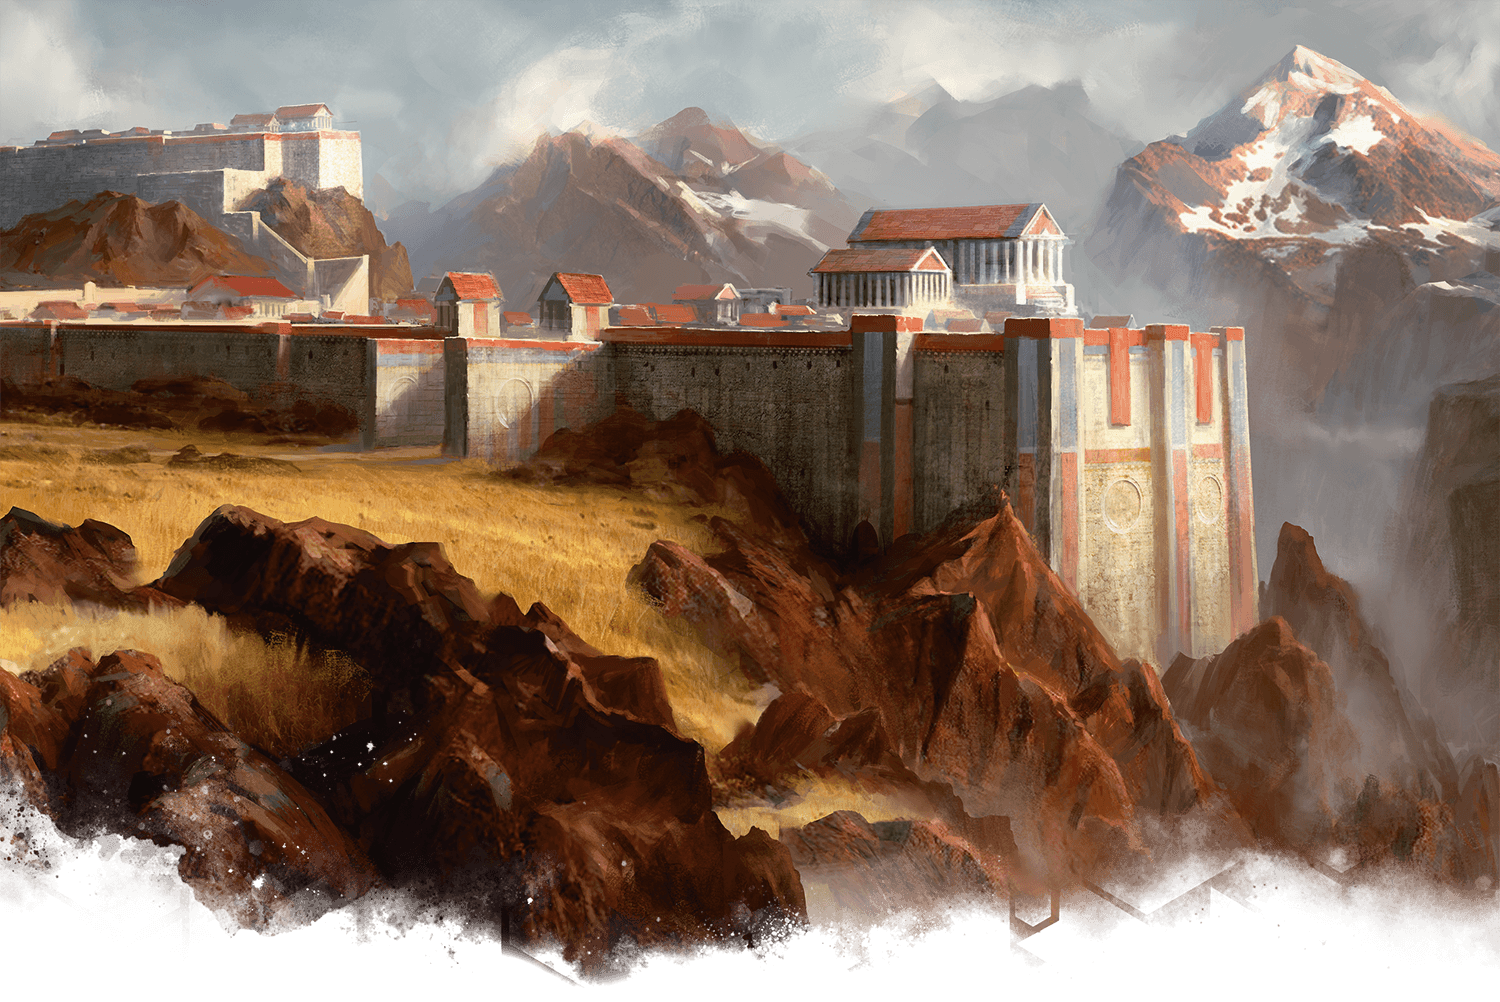
\includegraphics[width=\pdfpagewidth]{02viphoger/img/10kolophon.png}};
        \end{tikzpicture}

        \vspace{12.5cm}

        The ancient practice is viewed as primitive but powerful, and Akhoans of any background might risk making a pilgrimage into the mountains to hear a flamespeaker's prophecies.

    \subsubsection{Servants and Serfs}
        Lektoi who complete their military service with honor often retire to the Kolophon or their family estates and go about the leisured life of aristocrats.
        Their households are run by a class of servants made up of lektoi who were unable or unwilling to undertake a military career.
        These servants lack citizenship's full privileges but retain a position of some honor thanks to their class.

        Below these servants, at the bottom of Akhosh's social hierarchy, are the serfs.
        Comprising the vast majority of Akhosh's population, the serfs largely reside outside the protection of the Kolophon, laboring to grow the staple crops that support Akhosh's citizens and its trade.
        A relatively small number of serfs are skilled artisans who manage to build a more prosperous life for themselves with their crafts.
        But even these wealthier serfs can't own the land they live on, and they enjoy few rights or legal protections.

        \pagebreak~
        \vspace{12cm}

    \subsubsection{Nongats in Akhosh}
        Akhosh maintains a standoffish—and often hostile—stance toward its neighbors, particularly the treb gats of Phoberos, the leonin of Oreskos, and the dratl irds of the Pheres band.
        Members of those peoples rarely find a warm welcome in Akhoash territory.
        However, Akhoans respect prowess, loyalty, and self-sacrifice, and might welcome any who embody such virtues.
        Some stratians also seek to learn the martial practices of other peoples, and might invite individuals or small communities to Akhosh to learn their ways.

        During the Iroan Games, everyone is welcome in the stadium.
        Thousands flock to the city to witness the competition, and some take up permanent residence, celebrating the outcome of one year's games until it's time to start watching the next.

\subsection*{Features of Akhosh}
    At the center of the polis of Akhosh rises the Kolophon, a mighty fortress and the seat of Akhoash power.
    This many-tiered structure perches upon a vast cliff, which drops into a deep canyon carved by the Tsher River.
    Nature and Akhoash ingenuity conspire to make the Kolophon one of the most intimidating fortresses in Viphoger.

    Beyond the polis stretch craggy hills and canyon walls broken by narrow stretches of arable plains.
    It is a nearly impassable landscape, save for a few roads hewn through passes.
    Residents claim that only a fool would attempt to invade the heartlands of Akhosh, yet Akhoashs obsessively guard against invasion nonetheless.

    Beyond its thick walls, the streets of Akhosh are dotted with towering statues of heroes.
    Red-tiled roofs soar over square-topped sandstone columns, and holy sites dedicated to Iroas, Purphoros, and Keranos, among the other gods, are many.
    The architecture is formidable, spare, and militaristic, thick with sharp, angular shapes.

    \subsubsection{Temple of Triumph at Akhosh}
        At the heart of the walled city is the huge stadium that hosts Viphoger's greatest sporting event, the Iroan Games.
        A grand temple of Iroas stands beside it, serving as the venue for award ceremonies.
        A wide plaza connects the stadium to the city's outer gates, offering plenty of room for celebration around the annual games.

        When the stadium isn't hosting the actual Iroan Games, it is still used daily for training and for lesser athletic events.
        Many of the buildings surrounding the stadium are dedicated to serving it: smaller training facilities, providers of athletic gear, stables, and other shops.

    \subsubsection{Citadel}
        The uppermost tier of the city, perched on a rocky outcropping at the northwestern corner of the Kolophon, is the great citadel.
        The Oromai (the ``watchers'' who maintain order and defend the Kolophon) are quartered within the citadel's imposing walls, and the monarch's palace is built atop it.
        Temples of Iroas, Heliod, and Keranos also adorn the top of the citadel, the latter commissioned by the late prince Cymede, built with an open roof to give them a clear view of stormy skies.

\subsection*{Akhosh's Surroundings}
    Arable land is scattered across small plateaus and valleys in Akhosh, meaning that the serf communities that farm the land are small and just as scattered.
    Volcanic rifts, landslides, and venomous animals make travel dangerous for anyone who doesn't know the terrain, and visitors wishing to avoid suspicion from patrolling stratians would be wise to stick to the roads.

    \begin{figure}[!t] % NOTE: Maybe do something to this image so it doesn't look so underwhelming.
        \centering
        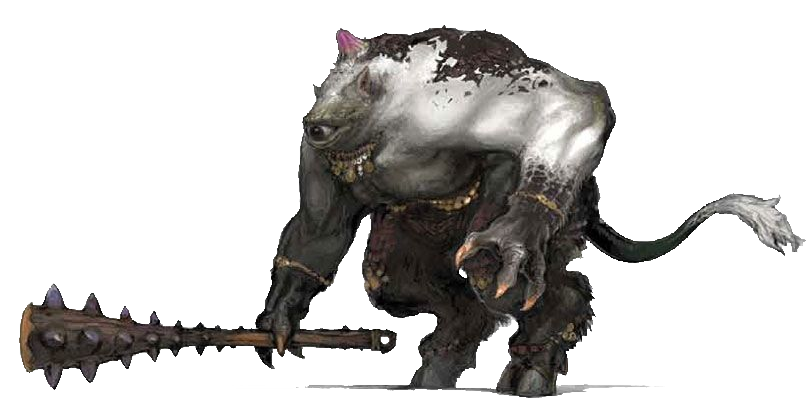
\includegraphics[width=0.48\textwidth]{02viphoger/img/10cyclops}
    \end{figure}

    \subsubsection{Outposts}
        The Alamon soldiers spend most of their time patrolling Akhosh's outlying areas, centering their patrols around scattered outposts.
        These serve as staging grounds for Alamon and Lukos units to prepare as they venture out to raid or guard against monsters and invaders.

        \subparagraph{One-Eyed Pass} The outpost in One-Eyed Pass serves to keep an Akhoash eye on the large cyclops population of the area, but the stratians also use the cyclopes to their advantage.
        Any time dangerous creatures come down from the mountains and pose a potential threat to Akhoash holdings, the Alamon harry the enemy and try to funnel them into the pass.
        The cyclopes of the pass viciously defend their territory against all intruders, weakening or even eliminating the danger before it can reach the Akhoash outpost, where the Lukos finish off any stragglers.

        \subparagraph{Pharagax Bridge} On the eastern border of Akhosh gapes a massive chasm rumored to descend all the way to the underworld and belch forth foul creatures.
        The great stone bridge that spans it is the only way into Akhosh from this direction.
        Stratians consider it a high honor to be assigned to guard the bridge.

        \subparagraph{Titan's Stairs} These stone ``stairs'', seemingly carved into the granite cliffs that protect Akhosh and haunted at all times by eerie, whistling winds, provide natural access to Akhosh.
        The stratians guard it fiercely and use it as a staging ground for invading the lowlands.

        \subparagraph{Katajthon Outposts} Several semipermanent encampments dot the rocky land between Akhosh and the rest of the Katajthon canyon.
        Fresh cadres of troops come here every month to relieve soldiers who are worn out by relentless assaults from raiders, fire-breathing dragons, and other threats.

        \subparagraph{Canyon Shrines} The Akhoashs believe that the gods are best worshiped at the places closest to the sky --- canyon peaks.
        Small temples and shrines are found throughout Akhoash territory.
        Some are tucked in caves or nestled in crevices or canyons, while others are bare altars exposed to the elements.

\pagebreak
